\chapter*{Направление прихода ШАЛ}
\addcontentsline{toc}{chapter}{Направление прихода ШАЛ}
\label{ch:intro}

\section*{Кластерный метод реконструкции направления прихода ШАЛ}
\addcontentsline{toc}{section}{Кластерный метод реконструкции направления прихода ШАЛ}
\label{sec:methods}


Направление прихода широкого атмосферного ливня \cite{shulzhenko2019} можно определить по относительным временам срабатывания детектирующих станций установки НЕВОД-ШАЛ, полагая фронт ШАЛ плоскостью, движущейся со скоростью света:
\begin{equation}
Ax+By+Cz+D=0
\end{equation}
уравнение плоскости, где коэффициенты A, B, C  одновременно не равны нулю.
Тогда расстояние между фронтом ШАЛ и детектирующей станцией можно искать, как
расстояние от точки до плоскости:
\begin{equation}
d = \frac{Ax+By+Cz+D}{\sqrt{A^2 + B^2 + C^2}} = ct
\end{equation}
где с - скорость света, t - относительное время срабатываня детектирующей станции.
Если искать вектор направление прихода широкого атмосферного ливня как единичный нормальный вектор, то коэффициенты плоскости нормируются на единицу:
\begin{equation}
A^2 + B^2 + C^2 = 1
\end{equation}
Тогда для поиска коэффициентов плоскости нужно найти минимум функционала:
\begin{equation}
F = \sum_{i=1}^{n} \left(\frac{ct_i - Ax_i - By_i - Cz_i - D}{c} \right)^2
\end{equation}
где n - число всех сработавших детектирующих станций установки невод ШАЛ в одном событии.

Для установки НЕВОД-ШАЛ направление прихода ШАЛ можно определять кластерный методом - усреднение направление прихода события по каждому отдельному сработавшему кластеру. \(t_i\) отсчитываются от момента срабатывания первой детектирующей станции кластера в событии, причем детектируюих станций одного кластера должно быть не менее трех. Зенитный и азимутальный углы \(\theta\) и \(\phi\) направление прихода ШАЛ определяются например как средние или медианное значения соответствующих углов в событии.

Зная, что детектирующие станции одного кластера установки НЕВОД-ШАЛ располагаются примерно на одном уровне, можно преобразовать функционал для кластерного метода к виду:
\begin{equation}
F = \sum_{i=1}^{n} \left(\frac{ct_i - Ax_i - By_i - D}{c} \right)^2
\end{equation}
а значение коэффициента С определяется из условия нормальности направляющего вектора
плоскости фронта широкого атмосферного ливня:
\begin{equation}
C = - \sqrt{1-A^2 - B^2}
\end{equation}

Были построены распределения разницы углов направления прихода ШАЛ совместных событий на установках ДЕКОР и НЕВОД-ШАЛ. Направление прихода события на установку НЕВОЛ-ШАЛ определялось как медианное направлений на сработавшие кластеры. На рисунке 11 представлено распределение \(\Delta \theta = \theta_{\text{Д}} - \theta_{\text{НШ}}\) (а) и распределение \(\Delta \phi = \phi_{\text{Д}} - \phi_{\text{НШ}}\) (б) по числу событий, где
\begin{itemize}
    \item \(\theta_{\text{Д}}, \phi_{\text{Д}}\) зенитный и азимутальный углы направления прихода события на установке ДЕКОР,
    \item \(\theta_{\text{НШ}}, \phi_{\text{НШ}}\) соответственно на НЕВОД-ШАЛ.
\end{itemize}

\begin{figure}[ht]
    \centering
    \subfloat[]{%
        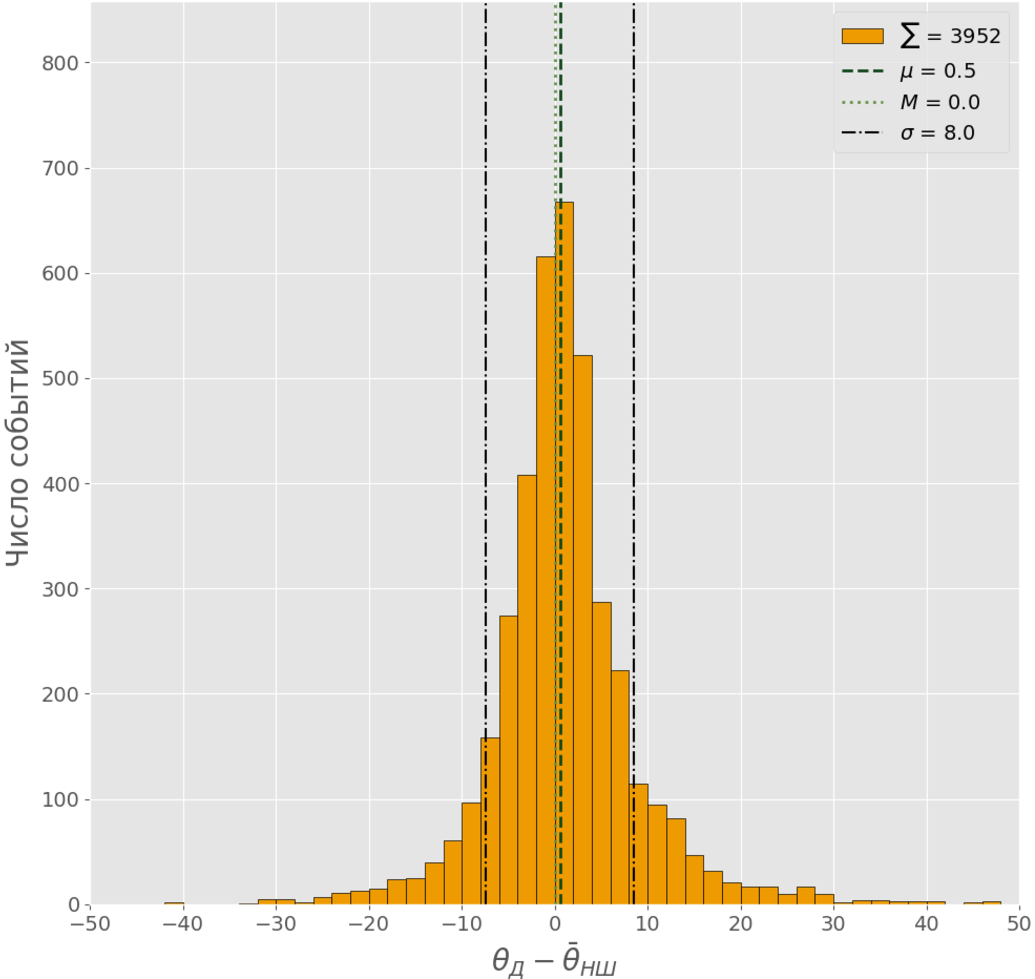
\includegraphics[height=8.5cm, keepaspectratio]{images/theta_hist.png}%
        \label{fig:muon_group1}%
    }%
    \subfloat[]{%
        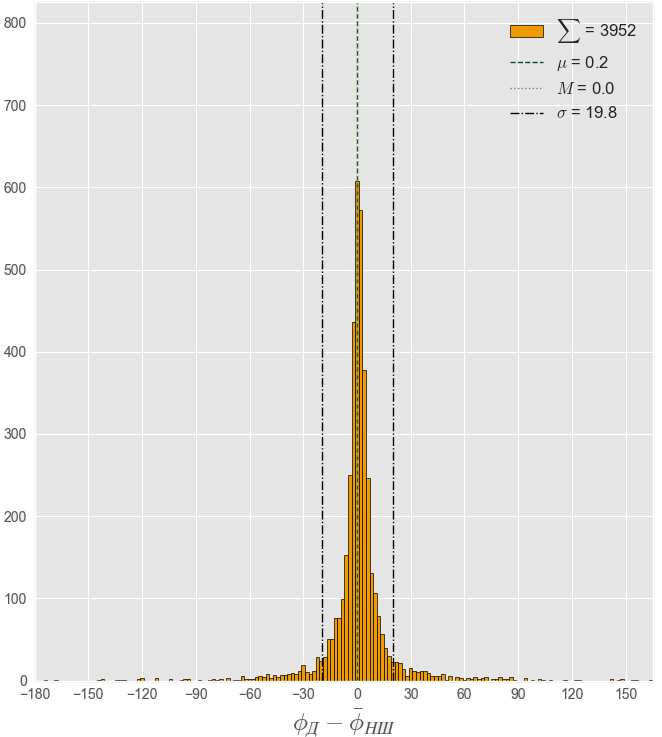
\includegraphics[height=8.5cm, keepaspectratio]{images/phi_hist.png}%
        \label{fig:muon_group}%
    }%

    \caption{распределение числа событий по разности углов направления прихода событий на установках ДЕКОР и НЕВОД-ШАЛ, зенитный угол (а), азимутальный угол (б)}
    \label{fig:muon_example}
\end{figure}


Считая, распределения нормальными можно полагать, что в пределах интервала \(\sigma_{\theta}\) = \(8\degree\) \((−\sigma_{\theta},+\sigma_{\theta})\) (где \(\sigma_{\theta}\) — стандартное отклонение) у 68\% событий зенитный угол \(\theta\) различается незначительно. Азимутальные углы имеют большее стандартное отклонение  \(\sigma_{\phi} = 20\degree\ \).

Большие выбросы на хвостах распределений объясняются низким числом сработавших кластеров НЕВОД-ШАЛ. На рисунке 12 представлено распределение угла между векторами направлений прихода событий ДЕКОР и НЕВОД-ШАЛ \(\angle(\mathbf{n_{\text{Д}}}, \mathbf{n_{\text{НШ}}})\)

\begin{figure}[ht]
    \centering
    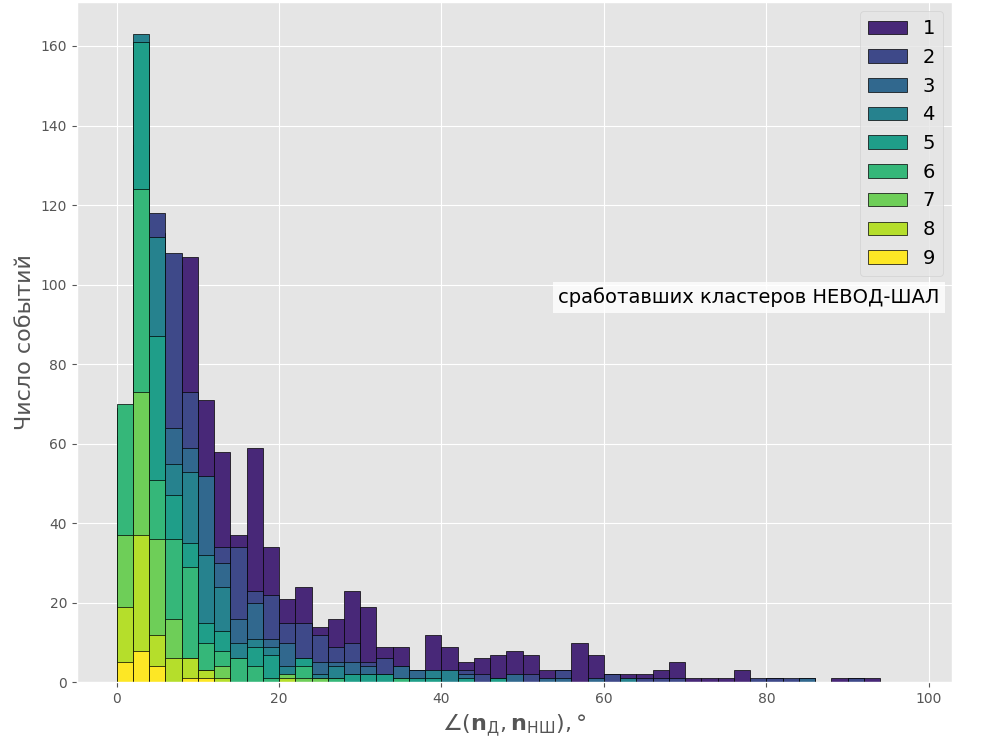
\includegraphics[width=1\textwidth]{images/vecs_angel.png}
    \caption{распределение числа событий по углу между векторами направления прихода событий на установках ДЕКОР и НЕВОД-ШАЛ}
    \label{fig:vecs_angel}
\end{figure}


Из распределения видно, что определение направления прихода события на НЕВОД-ШАЛ сходится к направлению на ДЕКОР при росте числа сработавших кластеров.

\section*{Вероятностная постановка задачи реконструкции}
\addcontentsline{toc}{section}{Вероятностная постановка задачи реконструкции}
\label{sec:methods}
Введу некоторые определения.
Пусть задано множество объектов \(X\), множество допустимых ответов \(Y\), и существует целевая функция \(\tilde{y} : X \to Y\), значения которой \(y = \tilde{y}(x_i)\) известны только на конечном подмножестве объектов \(\{x_1,...,x_l\} \subset X\). Задача обучения по парам \((x_i, y_i)\) заключается в том, чтобы по выборке \(X^l\) восстановить зависимость \(\tilde{y}\), то есть построить решающую функцию \(a : X \to Y\) , которая приближала бы целевую функцию \(\tilde{y}\), причём не только на  \(\{x_1,...,x_l\}\), но и на всём множестве X.

Решающая функция \(a\) должна допускать эффективную компьютерную реализацию, по этой причине буду называть её алгоритмом.

Признаком \(f\) объекта \(x\) будет результат измерения некоторой характеристики объекта. Формально признаком называется отображение \(f : X \to D_f\) , где \(D_f\)
множество допустимых значений признака.

В задаче реконструкции направления прихода ШАЛ в роли объектов выступят совместные события на установках. Признаки могут характеризовать координаты ДС, времена срабатываний ДС, задержки срабатывания ДС, положения мюонных пиков ДС, темпы счета ДС за определенный период и так далее, а в роли ответов выступают направления прихода событий ШАЛ.

Данные могут быть неточными, поскольку измерения значений признаков \(f_j(x)\) и целевой зависимости \(\tilde{y}\) обычно выполняются с погрешностями. Данные могут быть неполными, поскольку измеряются не все мыслимые признаки, а лишь физически доступные для измерения или например измерение времени срабатываний ДС может просто отсутствовать, если станция не сработала. В таком случае \(\tilde{y}\), строго говоря, не является функцией. Можно попробовать устранить эту некорректность с помощью вероятностной постановки задачи.

Вместо существования неизвестной целевой зависимости \(\tilde{y}\) предположим существование неизвестного вероятностного распределения на множестве \(X \times Y\)
с плотностью \(p(x, y)\), из которого случайно и независимо выбираются \(l\) наблюдений
\(X^l = (x_i, y_i)^{l}_{i=1}\). Такие выборки называются простыми.

Вероятностная постановка задачи считается более общей, так как функциональную зависимость \(\tilde{y}\) можно представить в виде вероятностного распределения \(p(x, y) = p(x)p(y|x)\), положив \(p(y|x) = \delta(y - \tilde{y})\), где \(\delta(z)\) - дельта-функция.

При вероятностной постановке задачи задаётся модель совместной плотности распределения объектов и ответов \(\xi(x, y, w)\), аппроксимирующая неизвестную плотность \(p(x, y)\). Затем определяется значение параметра \(w\), при котором выборка данных \(X_l\) максимально правдоподобна, то есть наилучшим образом согласуется с моделью плотности. Если наблюдения в выборке \(X_l\) независимы, то совместная плотность распределения всех наблюдений равна произведению плотностей \(p(x, y)\) в каждом наблюдении: \(p(X_l) = p((x_1,y_1, ..., x_l, y_l))= p(x_1,y_1) \cdot ... \cdot p(x_l,y_l)\). Подставляя вместо \(p(x, y)\) модель плотности \(\xi(x, y, w)\), получаем функцию правдоподобия
\begin{equation}
L(w, X^l) = \prod_{i=1}^l \xi(x_i,y_i,w)
\end{equation}
Чем выше значение правдоподобия, тем лучше выборка согласуется с моделью. Значит, нужно искать значение параметра \(w\), при котором значение \(L(w, X^l)\) максимально - принципом максимума правдоподобия.

Вместо максимизации \(L\) удобнее минимизировать функционал − \(\ln{L}\), поскольку
он имеет вид суммы:
\begin{equation}
-\ln{L(w, X^l) = - \sum_{i=1}^l \ln{\xi(x_i,y_i,w)} \to min}
\end{equation}
Пусть задана модель \(a(x, w)\), примем дополнительное вероятностное предположение,
что ошибки \( \varepsilon(x, w) = a(x, w) - \tilde{y}\) имеют нормальное распределение 
\(N(\varepsilon, 0, \sigma^2) = \frac{1}{\sigma \sqrt{2\pi}}\exp(-\frac{\varepsilon^2}{2\sigma^2})\) с нулевым средним и дисперсией \(\sigma^2\). Тогда модель плотности имеет вид
\begin{equation}
\xi(x,y,w) = p(x)\xi(y|x,w) = p(x)N(a(x, w) - \tilde{y};0,\sigma^2)
\end{equation}
Отсюда следует, что вероятностная функция потерь совпадает с квадратичной с точностью до констант \(C_0\) и \(C_1\), не зависящих от параметра \(w\)
\begin{equation}
-\ln{\xi(x,y,w)} = - \ln{p(x)N(a(x,w) - \tilde{y}(x);0,\sigma^2)} = C_0 + C_1(a(x,w) - \tilde{y}(x))^2
\end{equation}
Постоянными слагаемыми можно пренебречь тогда оказывается, что максимизация функции правдоподобия равносильна минимизации
\begin{equation}
\sum_{i=1}^l(\tilde{y}(x_i) - a(x_i, w))^2
\end{equation}
получилась неотрицательная функция, характеризующая величину реднеквадратичной ошибки алгоритма \(a\) на объекте \(x\).

Для построения решающей функции буду использовать многослойную нейронная сеть -  сложную дифференцируемуя функцию, задающая отображение из исходного признакового пространства в пространство ответов, все параметры которой могут настраиваться одновременно и взаимосвязанно. Многослойные сети можно настраивать градиентными методами, несмотря на огромное количество весовых коэффициентов. Хотя количество операций, необходимых для вычисления градиента, обычно возрастает пропорционально размерности, то есть числу весовых коэффициентов, этого удаётся избежать благодаря аналитическому дифференцированию суперпозиции с сохранением необходимых промежуточных величин - методу обратного распространения ошибок \cite{lecun1988theoretical}.

Рассмотрю многослойную сеть, в который каждый нейрон предыдущего слоя
связан со всеми нейронами последующего слоя. Введу следующие обозначения. Пусть выходной слой состоит из \(M\) нейронов с функциями активации \(\sigma_m\) и выходами (ответами) \(a^m\), \(m=1,...,M\). Перед ним находится скрытый слой из \(H\) нейронов с функциями активации \(\sigma_h\) и и выходами \(u_h\), \(h=1,...,H\). Веса cвязей между \(h\)-м нейроном скрытого слоя и \(m\)-м нейроном выходного слоя будем обозначать через \(w_{hm}\). Перед этим слоем может находиться либо входной слой признаков, либо ещё один скрытый слой с выходами \(v^j\), \(j=1,...,J\) и весами \(w_{jh}\). В общем случае число слоёв может быть произвольным. Если сеть двухслойная, то \(v^j\) есть просто \(j\)-й признак: \(v^j(x)=f_j(x)=x^j\), и \(j=n\). Обозначу через \(w\) вектор всех весов сети. Пример многослойной сети с одним скрытым слоем представлен на рисунке 13. 
\begin{figure}[ht]
    \centering
    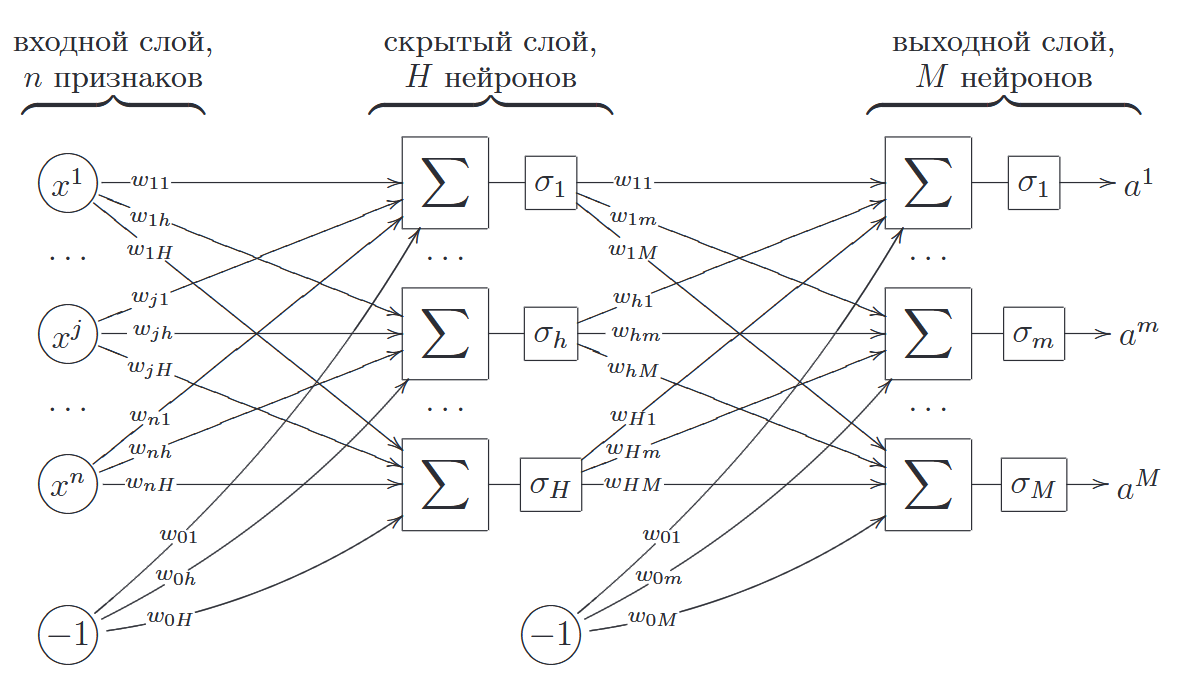
\includegraphics[width=1\textwidth]{images/nn.png}
    \caption{Многослойная сеть}
    \label{fig:nn}
\end{figure}

Выходные значения сети на \(x_i\) вычисляются как суперпозиция:
\begin{equation}
a^m(x_i) = \sigma_m \left(\sum_{h=0}^H w_{hm} u^h(x_i) \right); \qquad
u^h(x_i) = \sigma_h \left(\sum_{j=0}^J w_{jh} v^j(x_i) \right)
\end{equation}

Зафиксирую \(x_i\) и запишу функцию среднеквадратичной ошибки
\begin{equation}
Q(w) = \frac{1}{2}\sum_{m=1}^M \left(a^m(x_i) - y^m_i \right)^2
\end{equation}
Частная производная \(Q\) по выходам нейронов выходного слоя:
\[
\frac{\partial Q(w)}{\partial a^m} = a^m(x_i) - y^m_i = \varepsilon^m_i
\]
Частная производная \(Q\) по \(a_m\) равна величине ошибки \(\varepsilon^m_i\) на \(x_i\). Частные производные по выходам скрытого слоя:
\[
\frac{\partial Q(w)}{\partial u^h} = \sum_{m=1}^M \left(a^m(x_i) - y^m_i \right)\sigma'_m w_{hm} = \sum_{m=1}^M \varepsilon^m_i \sigma'_m w_{hm} = \varepsilon^h_i
\]
Получается ошибка сети на скрытом слое \(\varepsilon^h_i\). \(\varepsilon^h_i\) вычисляется по \(\varepsilon^m_i\), если запустить сеть «задом наперёд», подав на выходы нейронов скрытого слоя значения \(\varepsilon^m_i \sigma'_m\), а результат \(\varepsilon^h\) получив на входе. При этом входной вектор скалярно умножается на вектор весов \(w_{hm}\), находящихся справа от нейрона, а не слева, как при прямом вычислении 

\begin{minipage}{0.4\textwidth}
  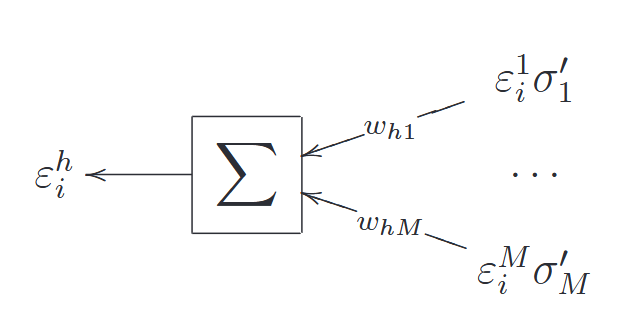
\includegraphics[width=\textwidth]{images/nn1.png}
\end{minipage}
\par
Градиент \(Q\) по весам:
\begin{equation}
\frac{\partial Q(w)}{\partial w_{hm}} = \frac{\partial Q(w)}{\partial a^m}  \frac{\partial a^m)}{\partial w_{hm}} = \varepsilon^m_i \sigma'_m u^h(x_i), \qquad m=1,...,M, \quad h=0,...,H;
\end{equation}
\begin{equation}
\frac{\partial Q(w)}{\partial w_{jh}} = \frac{\partial Q(w)}{\partial u^h}  \frac{\partial u^h)}{\partial w_{jh}} = \varepsilon^h_i \sigma'_h v^j(x_i), \qquad h=1,...,H, \quad j=0,...,J;
\end{equation}
и так далее для каждого слоя. Если слоёв больше двух, то остальные частные производные вычисляются аналогично - обратным ходом по слоям сети справа налево.

С помощью нейросети легко создать модель, которая предсказывает сразу и зенитный \(\theta\), и азимутальный \(\phi\) угол направления прихода ШАЛ. Достаточно сделать, чтобы последнее представление было матрицей \(B \times M\), где \(B\) - число объектов, а \(M\) — количество предсказываемых чисел. И тогда можно минимизировать фунцию по всей матрице \(B \times M\).

Для проверки работы модели были рассчитаны относительные времена срабатывания  детектирующих станций установки НЕВОД-ШАЛ для заданных углов направления прихода событий \(\theta \in [0,\frac{\pi}{2}]\), \(\phi \in [0, 2\pi)\) - пусть в момент времени \(t=0\) соответствует положению фронта, когда он проходит через начало координат \(\textbf{r}=[0,0,0]\), для ДС, время срабатывания определяется относительно этого момента как 
\(t_i = - \frac{\mathbf{r}_i \cdot \mathbf{v}}{c}\), где 
\begin{itemize}
    \item \(\mathbf{r_i}\) радиус-вектор к ДС,
    \item \(\mathbf{v} = [\sin{\theta}\cos{\phi}, \sin{\theta}\sin{\phi}, \cos{\theta}]\) вектор направления прихода ШАЛ,
    \item \(c\) скорость света.
\end{itemize}

Для приближения соответствия данных к реальным наблюдаемым событиям на установке НЕВОД-ШАЛ учтено, что не все детектирующие станции могут срабатывать. На рисунке 14 представлено распределение разницы предсказаний модели и заданных значений углов \(\theta\) и \(\phi\) для 7080 разыгранных событий, не участвующих в построении решающей функции.
\begin{figure}[ht]
    \centering
    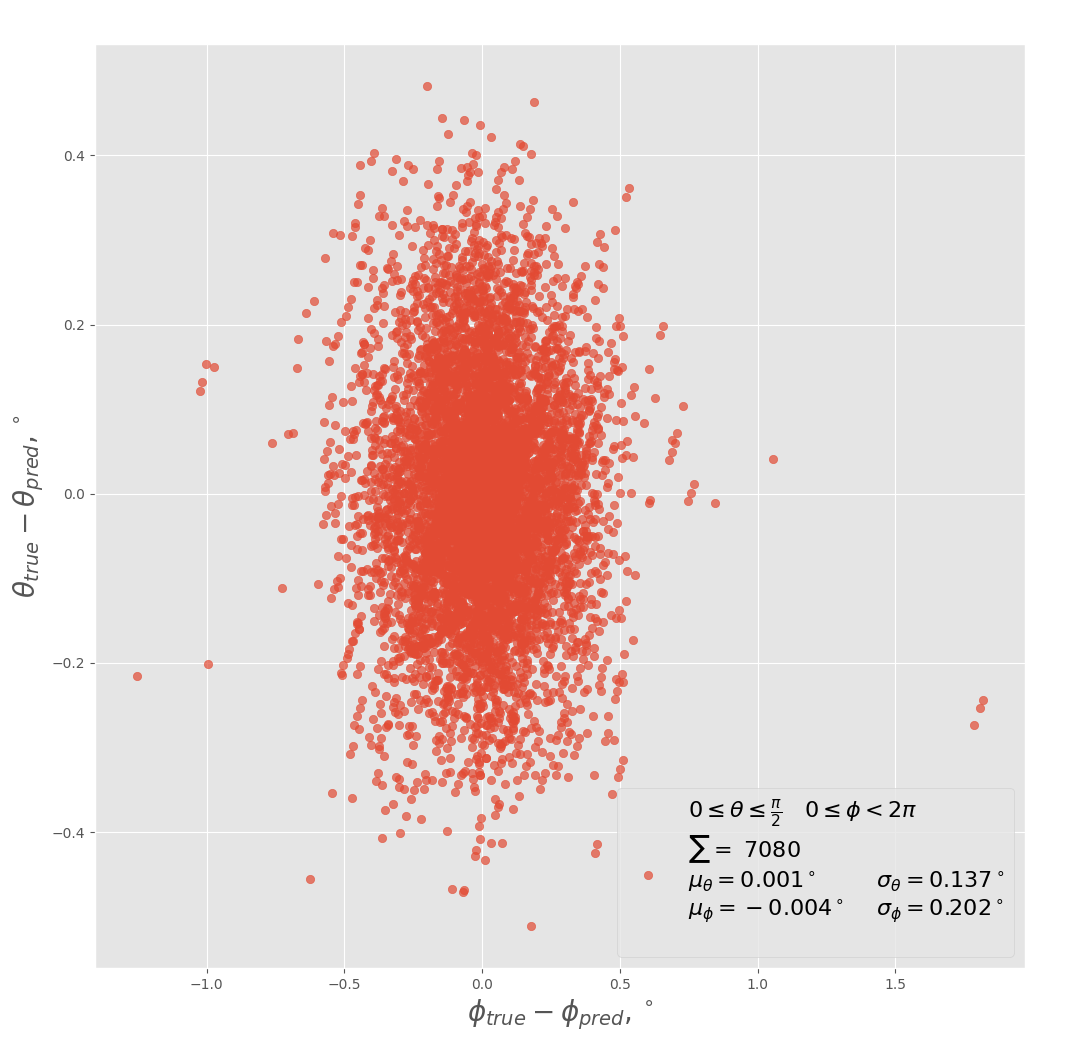
\includegraphics[width=0.95\textwidth]{images/test_theta_vs_phi_diff.png}
    \caption{Распределение разницы предсказаний модели и заданных значений углов \(\theta\) и \(\phi\) направлений прихода ШАЛ}
    \label{fig:nn}
\end{figure}

Для предсказания значений \(\theta\) и \(\phi\) найденных совместных событий на установках ДЕКОР и НЕВОД-ШАЛ были создан синтетический набор данных откликов ДС. Для учета задержек срабатывания ДС и влияние системных и статистических факторов на результаты измерений был добавлен шум, соответствующий значениям распределения разницы времени откликов, вычисленных по направлению прихода совместного события на установку ДЕКОР, и реальным временем срабатывания ДС установки НЕВОД-ШАЛ для того же события. На рисунке 15 и 16 представлены значения зенитного угла \(\theta\) и \(\phi\) найденных совместных событий, определенные по данным установки ДЕКОР, НЕВОД-ШАЛ и моделью. 
\begin{figure}[ht]
    \centering
    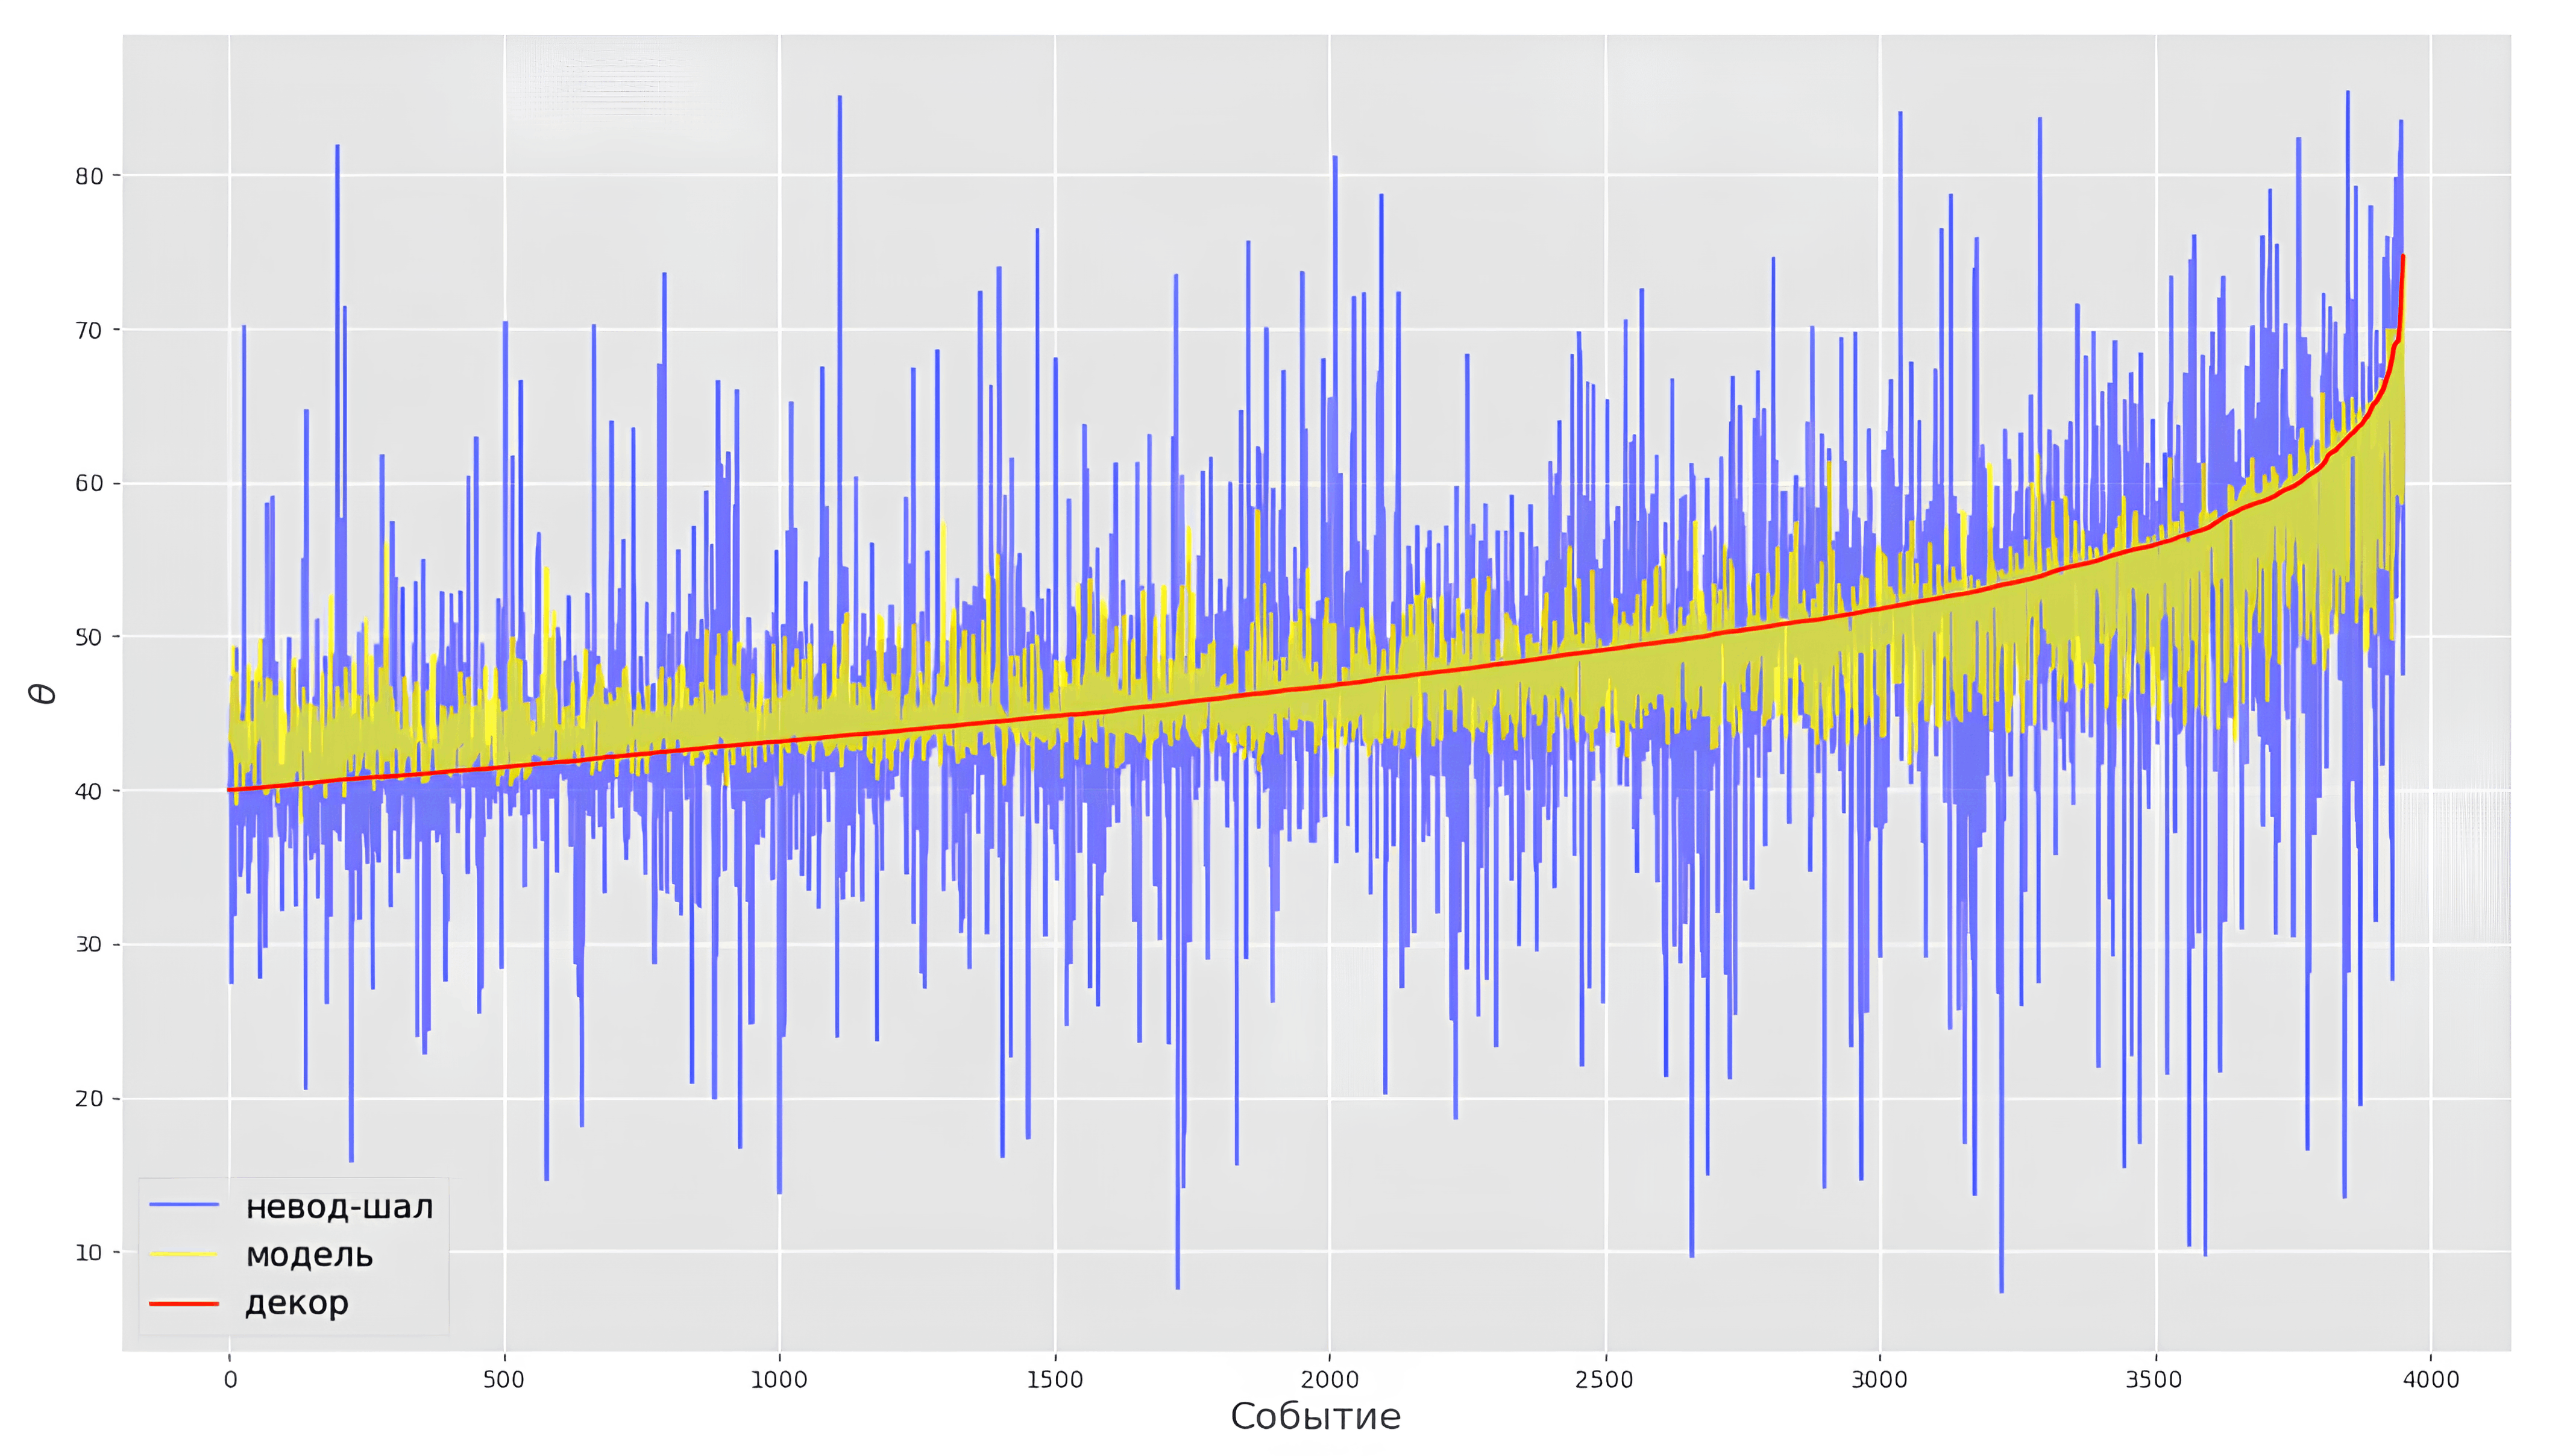
\includegraphics[width=1\textwidth]{images/theta_3_1.png}
    \caption{Значения зенитного угла \(\theta\) найденных совместных событий, определенные по данным установки ДЕКОР (красный), НЕВОД-ШАЛ (синий) и моделью (желтый)}
    \label{fig:theta}
\end{figure}

\begin{figure}[ht]
    \centering
    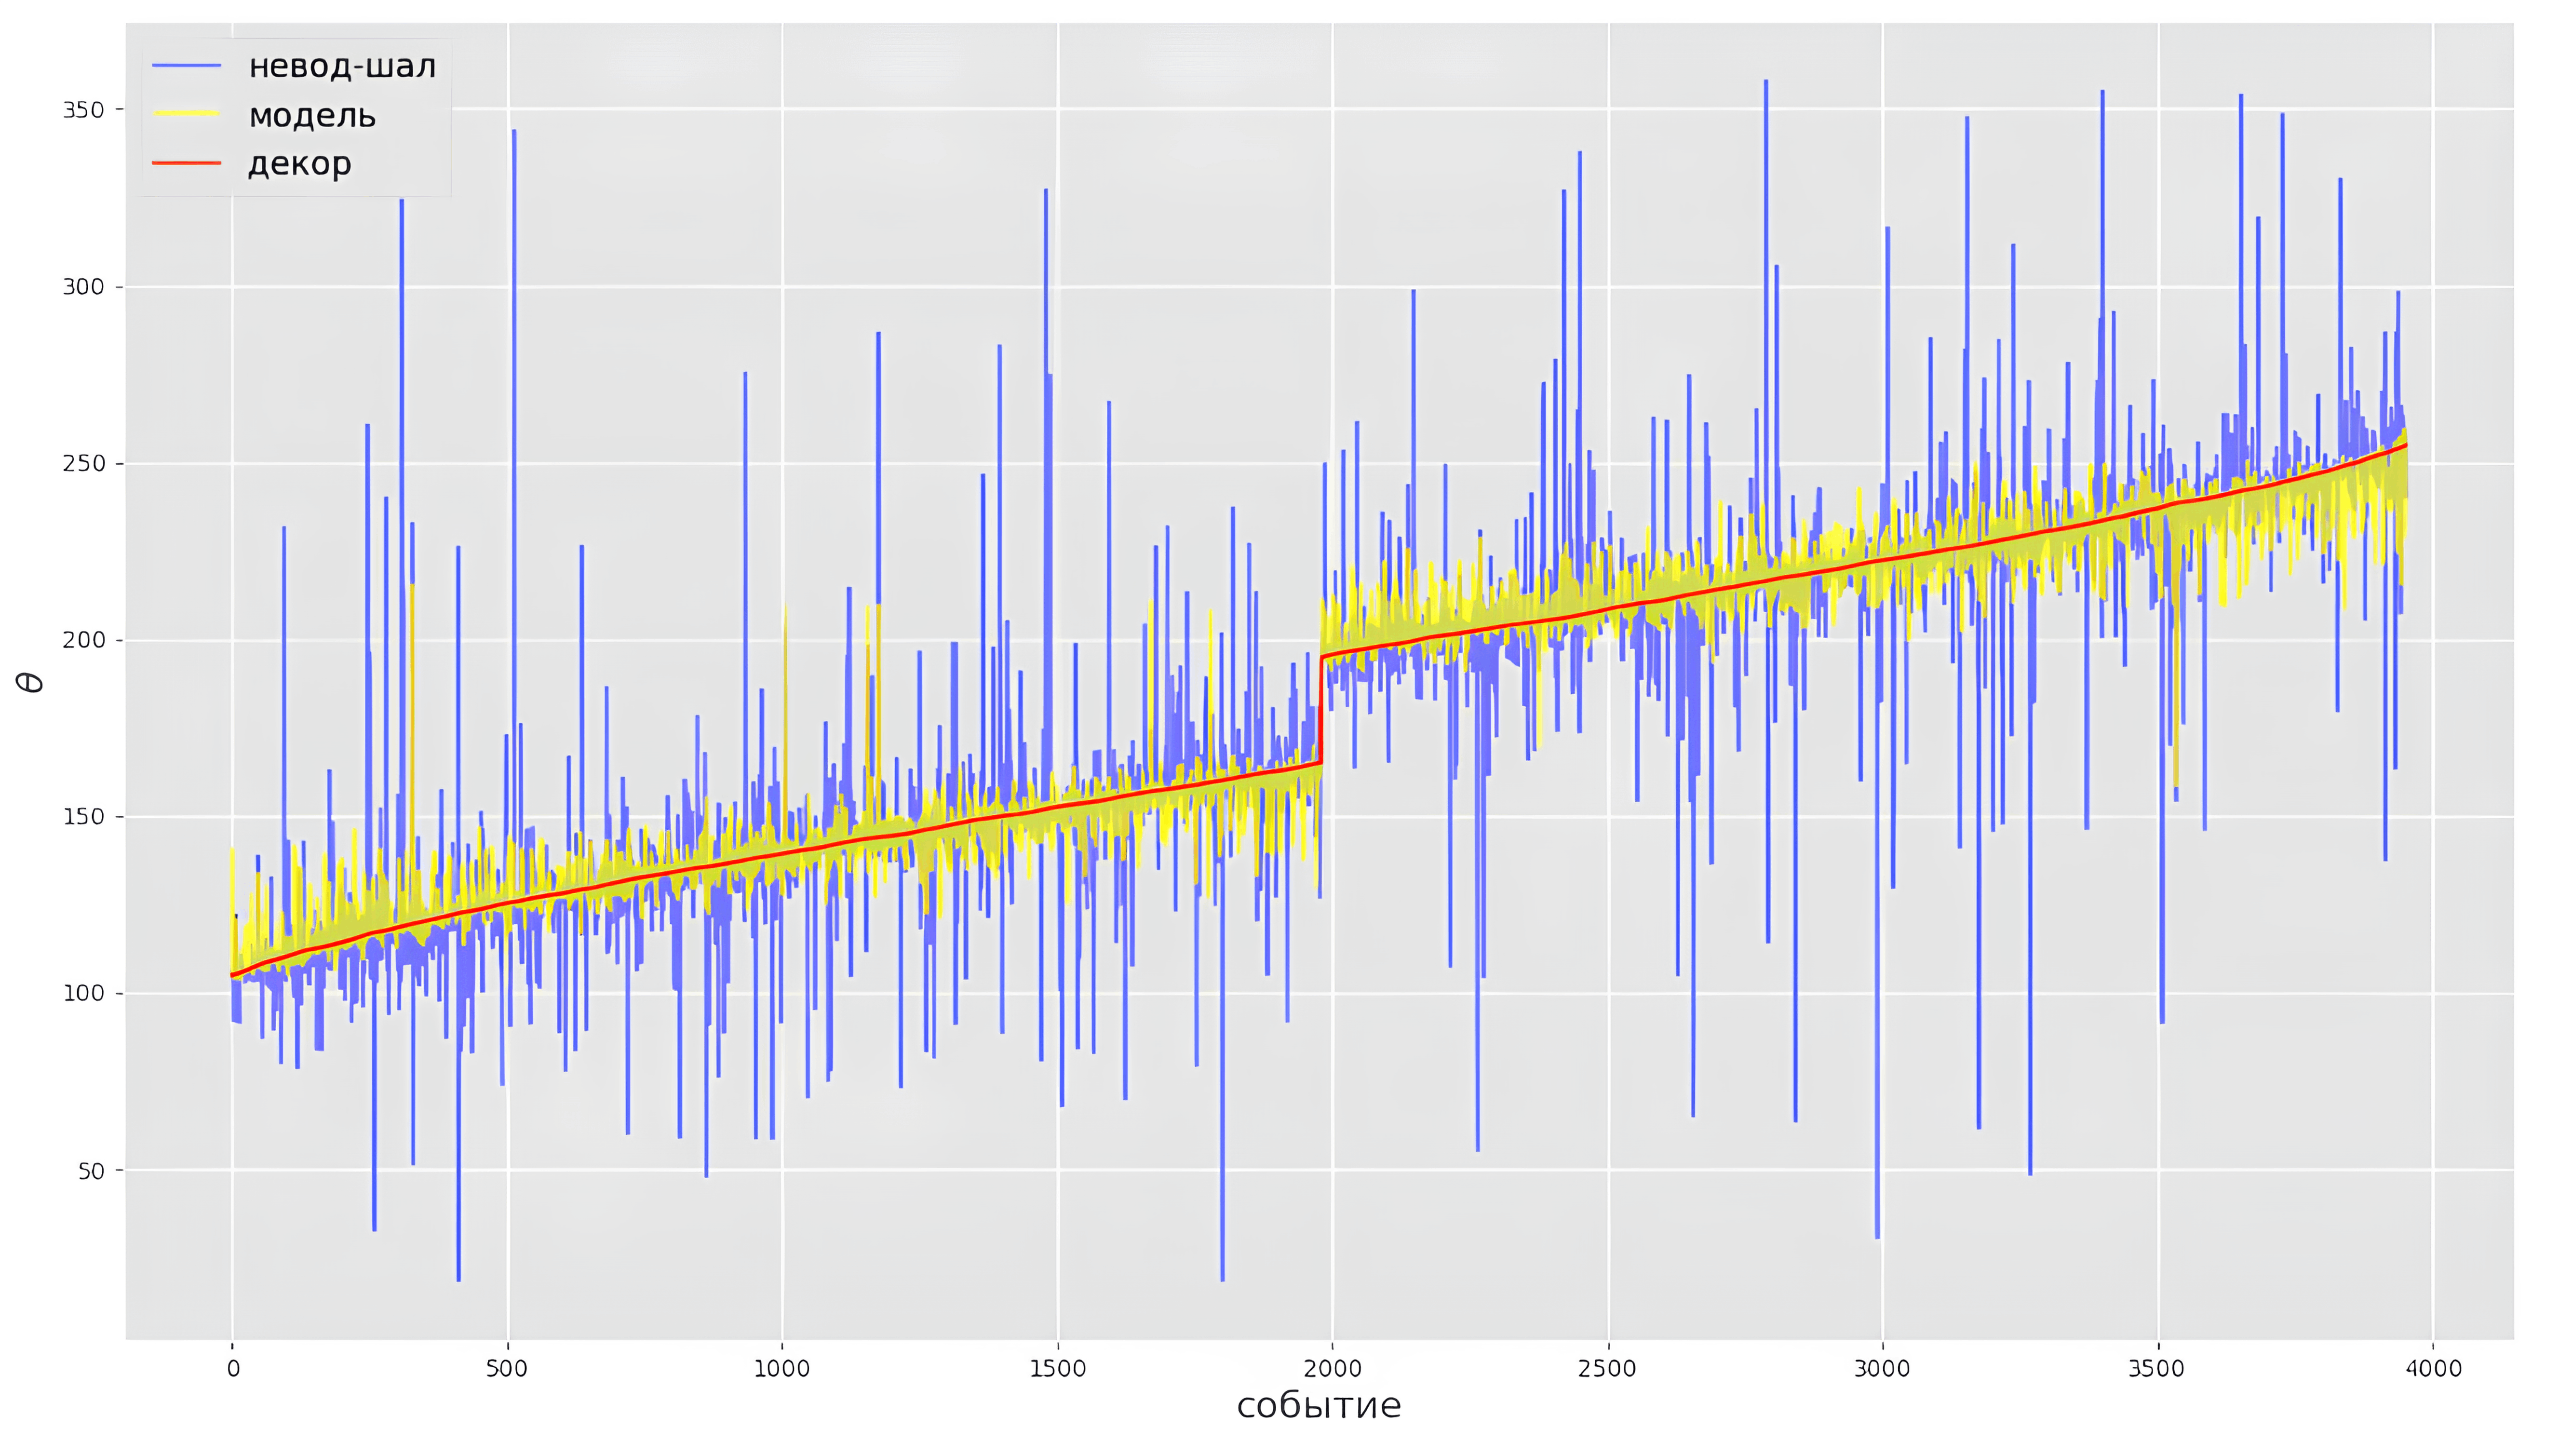
\includegraphics[width=1\textwidth]{images/phi_3_1.png}
    \caption{Значения азимутального угла \(\phi\) найденных совместных событий, определенные по данным установки ДЕКОР (красный), НЕВОД-ШАЛ (синий) и моделью (желтый)}
    \label{fig:phi}
\end{figure}

\clearpage 
Квадратичный корень из средней квадратичной ошибки предсказаний модели и значениями ДЕКОР:
\[
RMSE = \sqrt{\frac{1}{N}\sum_{i=1}^N \| \mathbf{y_{\text{Д}}} - \mathbf{y_{\text{М}}} \|^2} = 5.8 \degree
\]
Для сравнения квадратичный корень из средне квадратичного расхождения значений ДЕКОР и НЕВОД-ШАЛ равен \(20.9\degree\).

Учитывая, что сходимость направления прихода события на установке НЕВОД-ШАЛ к направлению прихода совместного события на установке ДЕКОР пропорциональна числу сработавших кластеров на НЕВОД-ШАЛ, можно обучать модель непосредственно на значениях направления прихода совместного события на установке ДЕКОР. В теоретическом плане, с увеличением объема выборки совместных событий на установках, а также с учетом регистрации групп мюонов, приходящих под любыми углами, возможно более точное реконструирование направления любого события, зарегистрированного установкой НЕВОД-ШАЛ. 
\endinput